% DME
% version 2018
%-------------------------------------------------------

\section{Introducci\'on}
\label{sec:DME.introduccion}

El equipo medidor de distancias %(DME, del ingl\'es: Distance Measuring Equipment)
\ac{DME}
 es un sistema electr\'onico que permite establecer la distancia entre \'este y una estaci\'on emisora, reemplazando a las radiobalizas en muchas instalaciones. Generalmente ligado a la aeron\'autica, el DME es uno de los sistemas de ayuda a la navegaci\'on habitualmente presentes en cualquier aeronave.

Proporciona una medici\'on de la distancia (seg\'un la velocidad) al suelo (groundspeed). La frecuencia est\'a comprendida entre 962 y 1213 MHz (banda UHF) de 200 canales, que puede trabajar con una \'unica frecuencia para el DME o estar asociado a otra radioayuda como un VOR, ILS o MLS. En equipos antiguos la frecuencia se selecciona sintoniz\'andolo en el equipo como una radio t\'ipica, pero en equipos actuales se selecciona autom\'aticamente al sintonizar la radioayuda a la que est\'a asociado.

Ya que un avi\'on dispone de dos frecuencias de navegaci\'on utilizables al mismo tiempo, el selector del DME permite indicar qu\'e equipo de navegaci\'on queremos que nos indique la distancia. Algunos tambi\'en disponen de la opci\'on HOLD, en la que al pasar de una lectura DME de un equipo a esa posici\'on guarda en la memoria la frecuencia que estaba usando, teniendo as\'i la posibilidad de cambiar de VOR, ILS o MLS en un HSI, RMI o RBI sin perder la medici\'on de la distancia anterior. Esta opci\'on es muy \'util en vuelos IFR en los que la salida est\'andar instrumental del aeropuerto (SID) requiere cambios de radioayuda frecuente pero se basa en una \'unica medici\'on de DME.

El \ac{DME} fue inventado en Australia por  Edward George ``Taffy'' Bowen mientras se desempe\~naba como Jefe de la Divisi\'on de Radiof\'isica en la  Commonwealth Scientific and Industrial Research Organisation (CSIRO). Otra versi\'on fue desarrollada por la Amalgamated Wireless Australasia Limited a principio de la d\'ecada de 1950 operando en la banda de los 200 MHz VHF. Esta versi\'on dom\'estica australiana se la denomina DME(D), de \emph{Domestic}, y la versi\'on adoptada por la OACI es la DME(I).

El sistema fue un desarrollo post-guerra del IFF (Identification Friend or Foe), identificador amigo-enemigo, utilizado en la Segunda Guerra Mundial, es un sistema de identificaci\'on criptogr\'afica. Dentro del campo militar, sirve para distinguir a aeronaves o a veh\'iculos enemigos de los que no lo son.

Su funcionamiento se basa en la respuesta a una interrogaci\'on hecha por otro sistema. En funci\'on de si la respuesta es correcta o no, se identificar\'a como amigo o enemigo.

\begin{figure}[!htb]
  \centering
  \subfigure[]{  
	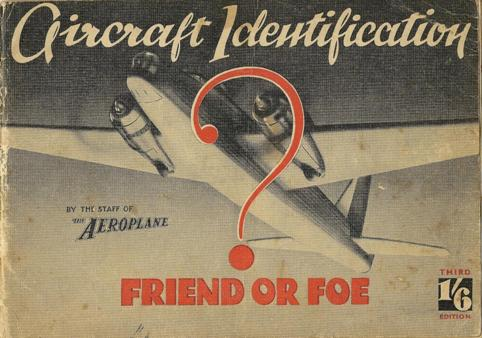
\includegraphics[width=0.45\textwidth]{Imagenes/06.04.dme.imagenes/iff.jpg}
	}
  \subfigure[]{  
	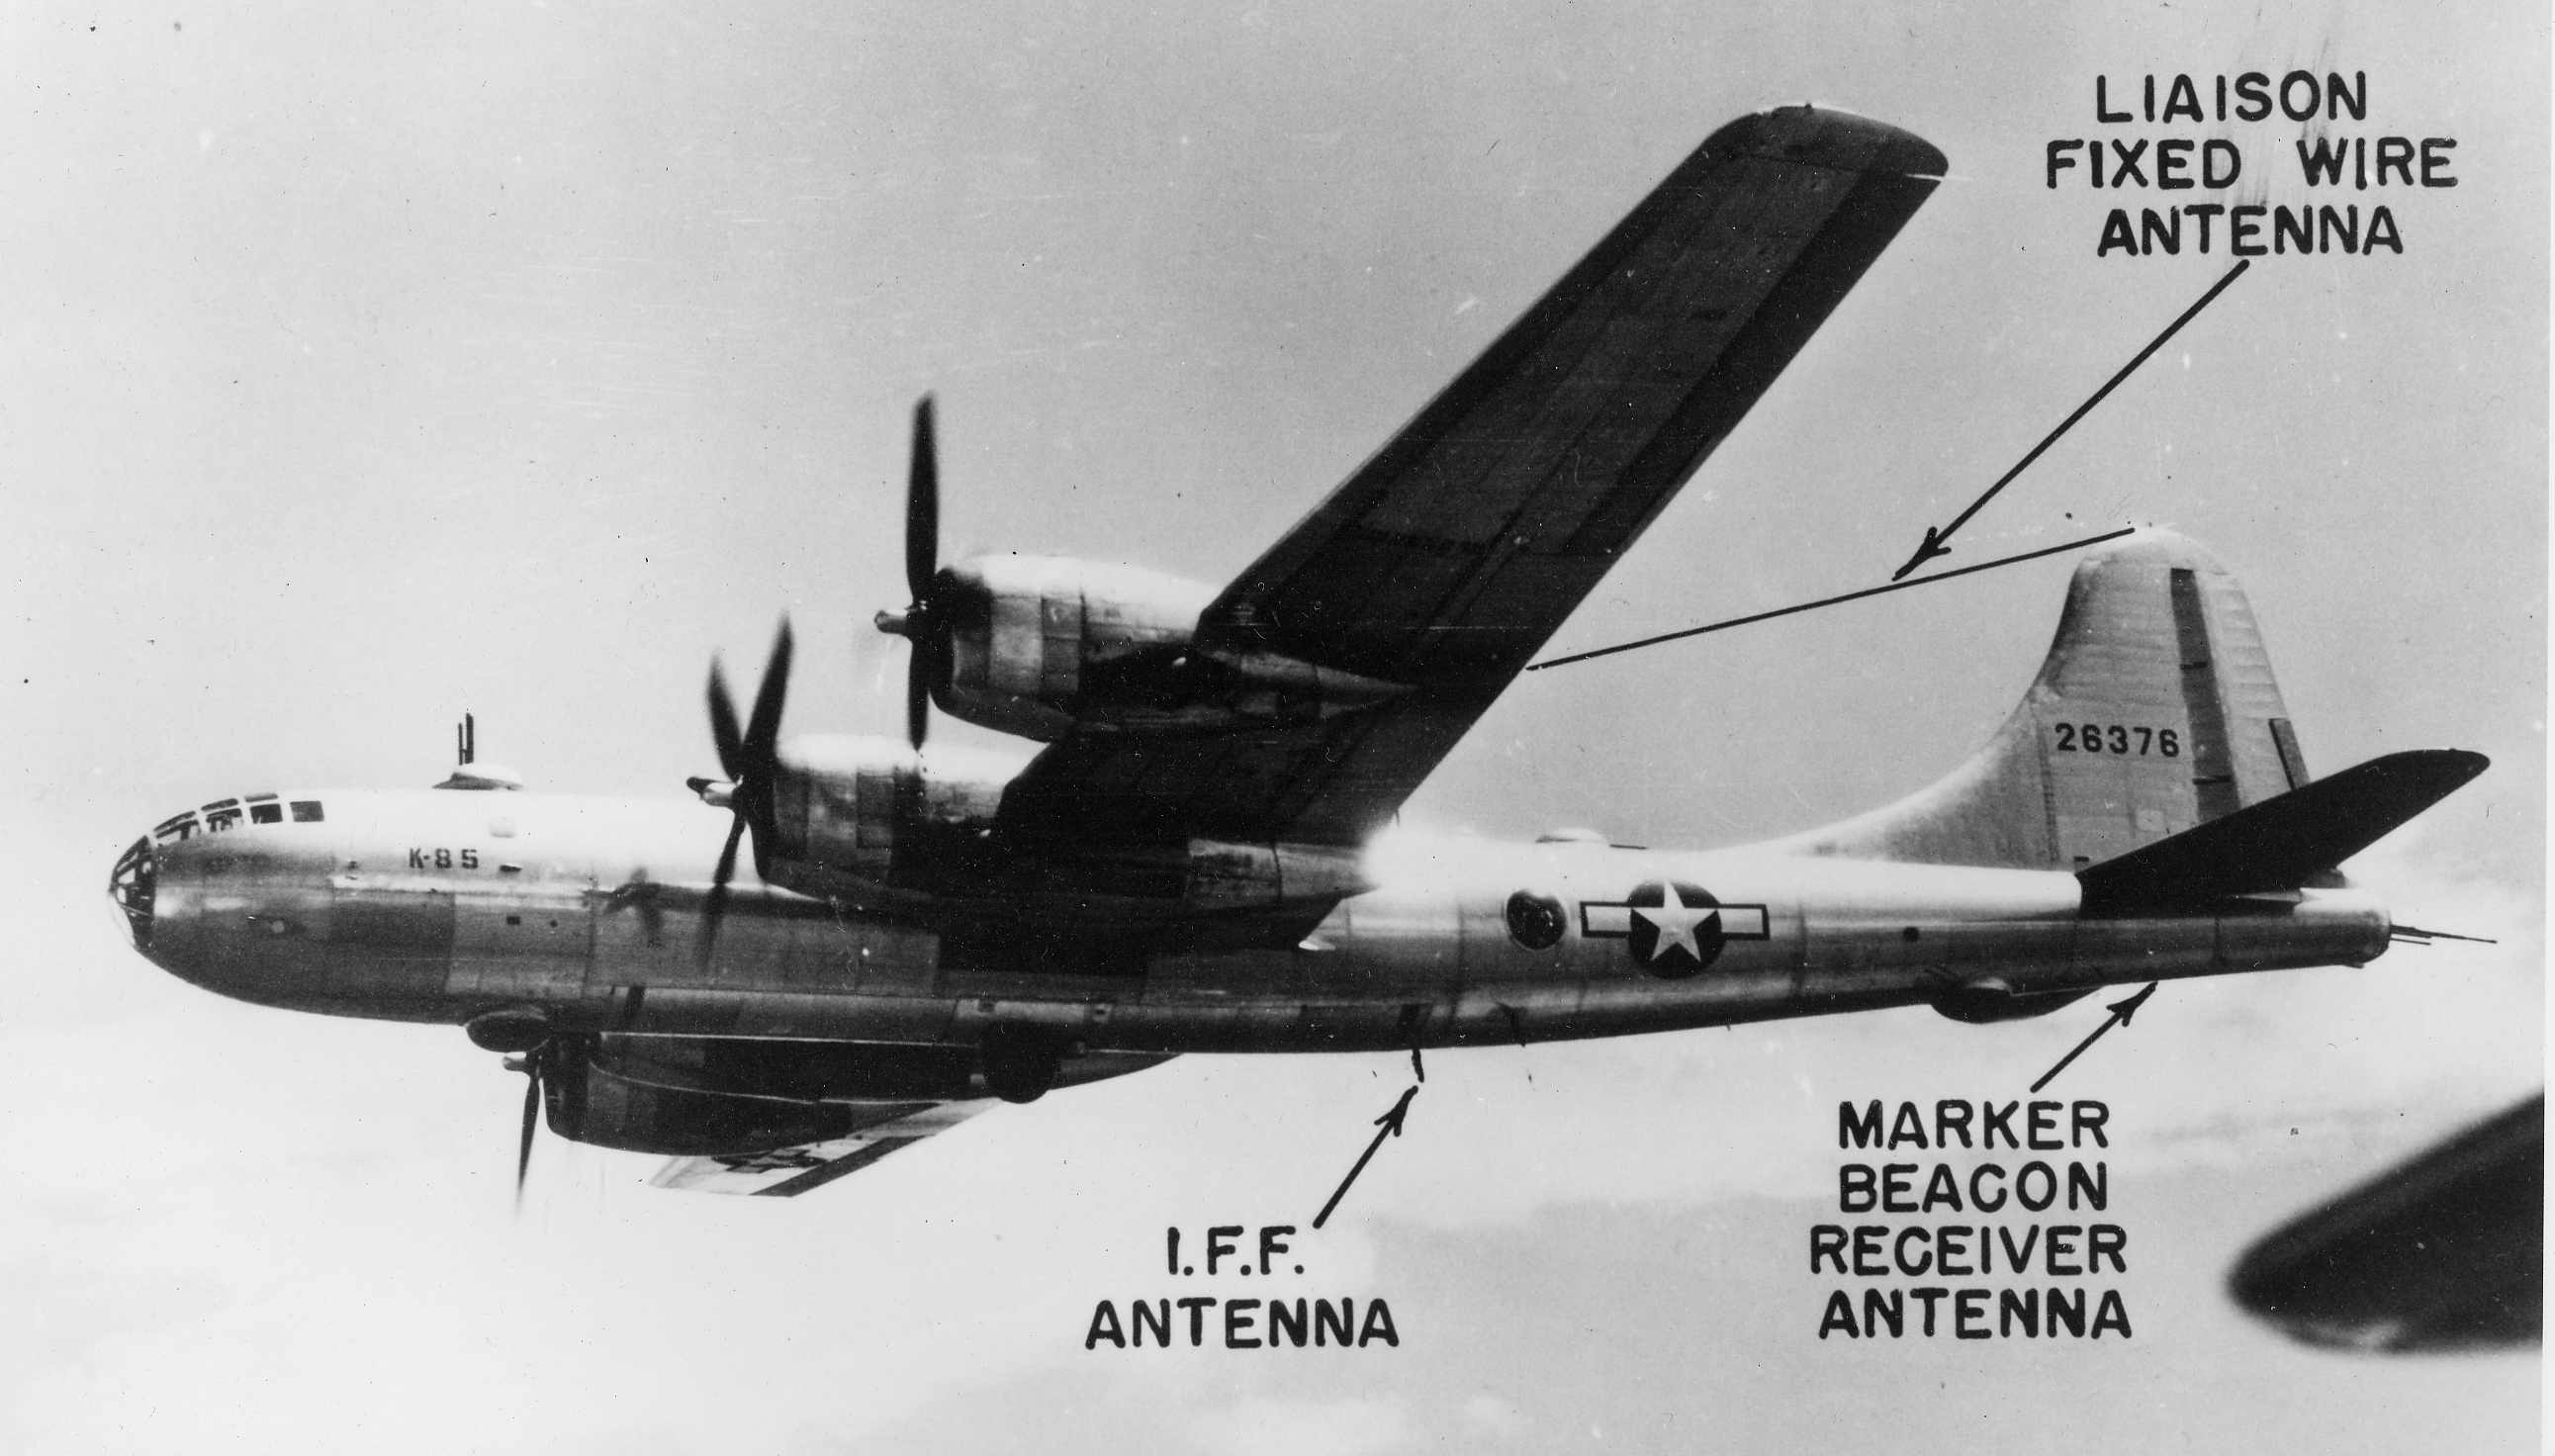
\includegraphics[width=0.45\textwidth]{Imagenes/06.04.dme.imagenes/B-29_antennas_port.JPG}
	}

  \caption{Sistema IFF}
  \label{fig:DME.sistema.iff}
\end{figure}


\section{Principio de funcionamiento}
\label{sec:DME.principio.funcionamiento}

El avi\'on interroga con una secuencia de pares de pulsos separados 12 $\mu$\,seg. El equipo de tierra que recibe esta se\~nal la retrasmite de nuevo con un retardo de 50 $\mu$\,seg. El equipo del avi\'on calcula el tiempo trascurrido desde que pregunt\'o, le descuenta 50 $\mu$\,seg y lo divide por dos. Este tiempo se multiplica por la velocidad de la luz (300 m/$\mu$\,seg), dando la distancia al equipo de tierra.

\begin{figure}[!h]
  \centering
  \includegraphics[width=0.6\textwidth]{Imagenes/06.04.dme.imagenes/how_to_dme_arc_Picture1.gif}
  \caption{Principio funcionamiento DME {\tiny fuente: \url{http://http://www.ivaoth.org/training/how_to/how_to_dme_arc.htm}}}
  \label{fig:DME.principio.funcionamiento}
\end{figure}

La distancia indicada por el equipo, denominada distancia oblicua, no corresponde a la distancia que separa a la aeronave de la estaci\'on en el plano horizontal, pero a distancias grandes es muy aproximada. No obstante al acercarse a la vertical de la estaci\'on, el error va aumentando y sobre la vertical, en el caso de que existiese cobertura, la distancia indicada ser\'ia igual a la altura.

Dado que son las aeronaves las que transmiten los pulsos de interrogaci\'on, puede darse el caso, y de hecho se da, que lo hagan varias a la vez. Estas interrogaciones llegar\'an al transpondedor que generar\'a y emitir\'a los pulsos de respuesta todos en la misma frecuencia. Entonces tenemos un mont\'on de pulsos en el espacio y cada aeronave tiene que encontrar la forma de distinguir los que son respuestas a sus interrogaciones para calcular su distancia a la estaci\'on.

La forma de distinguirlos consiste en generar los pulsos de interrogaci\'on con una frecuencia de repetici\'on de pulsos cambiante, es decir, separando los pares de pulsos por un tiempo aleatorio pero que queda memorizado en el interrogador. Al recibir los pulsos de respuesta, se van comparando con la secuencia memorizada y cuando coinciden se sabe que son los correspondientes a las interrogaciones propias. Entonces solo queda calcular la distancia por el m\'etodo descrito.

Lo indicado anteriormente resuelve el problema para el interrogador, pero no para el transpondedor de tierra cuya capacidad de respuestas no es ilimitada. Con el fin de aumentar el n\'umero de aeronaves que pueden obtener informaci\'on de distancia a la vez sin saturar la capacidad del transpondedor, se programa a los interrogadores para que hagan su trabajo en dos fases distintas:

\begin{itemize}
	\item \textbf{Funci\'on B\'usqueda:} es la fase inicial cuando se sintoniza una estaci\'on de tierra. En ella el n\'umero de interrogaciones es muy elevado, unas 150 por segundo, para intentar establecer un valor inicial de la distancia con un error menor de 20 NM. Esta fase no durar\'a m\'as de 20 segundos.
        \item \textbf{Funci\'on Seguimiento:} una vez que el interrogador a determinado la distancia aproximada a la que se encuentra de la estaci\'on, se entra en esta fase en la que el ritmo de interrogaciones desciende hasta unas 25 por segundo. Ahora el objetivo es aumentar la precisi\'on con que se conoce la distancia medida y realizar un seguimiento de la aeronave en su desplazamiento.
\end{itemize}.

Teniendo en cuenta el n\'umero m\'aximo de interrogaciones en cada una de las dos fases, se establece un n\'umero m\'aximo total de 100 aeronaves que pueden utilizar una estaci\'on DME de forma simult\'anea. Con estas 100 aeronaves, el transpondedor estar\'ia transmitiendo 2700 pares de pulsos por segundo.

Adem\'as de las respuestas a las interrogaciones recibidas, el transpondedor transmite una identificaci\'on formada por tres letras en c\'odigo Morse e id\'entica a la transmitida por la estaci\'on de informaci\'on acimutal (Localizador o VOR) a la que est\'e asociado. Esta identificaci\'on consiste en la transmisi\'on de pares de pulsos a raz\'on de 1350 pares por segundo. Los pares de pulsos se transmiten cada aproximadamente 40 segundos.

Con el fin de optimizar el funcionamiento del transmisor del transpondedor, sobre todo de los antiguos que funcionaban a v\'alvulas, este se dise\~na para una transmisi\'on continua m\'inima de 700 pares por segundo, excepto durante la transmisi\'on de los pares de pulsos de interrogaci\'on. Cuando el n\'umero de aeronaves est\'a por debajo de este valor m\'inimo, el transpondedor genera unos pulsos de relleno llamados \emph{squitter} que sirven para mantener constante el ciclo de trabajo del transmisor. Es decir, aunque no haya ninguna aeronave interrog\'andolo, el transpondedor siempre est\'a transmitiendo pulsos, bien de identificaci\'on o squitter.

Resumiendo todo lo anterior, se puede decir que en el tren continuo de pulsos transmitidos por el transpondedor se encuentran de forma aleatoria:

\begin{itemize}
	\item Respuestas a interrogaciones
	\item Pares de pulsos de identificaci\'on
	\item Pulsos de squitter.
\end{itemize}


En caso de que el n\'umero de aeronaves que est\'an interrogando a la vez llegase al 90\% del valor m\'aximo de 2700 pares por segundo, el sistema de supervisi\'on del transpondedor disminuye la sensibilidad del receptor para eliminar las interrogaciones de aeronaves muy distantes que al llegar m\'as d\'ebiles se rechazar\'an en el receptor. Llevamos mucho rato hablando de los pares de pulsos sin todav\'ia haber aclarado un poco sus caracter\'isticas, as\'i que vamos a hacerlo ahora. Como podemos ver en la figura, cada interrogaci\'on y su correspondiente respuesta est\'a formada por una serie de pares de pulsos de radiofrecuencia. La duraci\'on de estos pulsos en los puntos de amplitud media es de 3.5 ms ( 1 microsegundo = 0.000001 s) y la separaci\'on entre los dos pulsos del par es de 12 ms tanto en la interrogaci\'on como en la respuesta en el caso de canales X. Con el fin de aumentar el n\'umero de canales dentro de la misma banda de frecuencias, OACI establece otros canales denominados canales Y en los cuales la separaci\'on entre pulsos es de 36 ms en la interrogaci\'on y 30 ms en la respuesta. La forma del pulso es la de una campana de Gauss, ver Figura \ref{fig:DME.modos.X.e.Y.grafico}.

\begin{figure}[!htb]
  \centering
  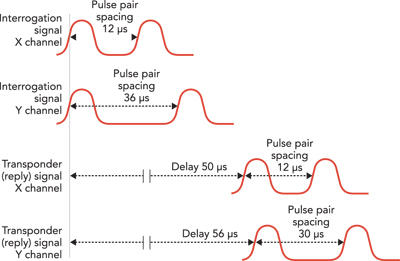
\includegraphics[width=0.6\textwidth]{Imagenes/06.04.dme.imagenes/dme-modos-x-y-graficos.jpg}
  \caption{Modos X e Y
{\tiny fuente: \url{http://www.tmworld.com/electronics-news/4386082/Signal-generator-power-sensor-test-DME-4386082
}}
}
  \label{fig:DME.modos.X.e.Y.grafico}
\end{figure}


\begin{figure}[!htb]
  \centering
  \includegraphics[width=0.6\textwidth]{Imagenes/06.04.dme.imagenes/dme-modos.gif}
  \caption{Modos X e Y
{\tiny fuente: \url{http://
aelmahmoudy.users.sourceforge.net/electronix/egair/radar.htm
}}
}
  \label{fig:DME.modos.X.e.Y}
\end{figure}

%In the upper diagram, if the pilot selects channel #1, on the X-Mode (1X) for example, then the aircraft DME will send its pulse pair interrogation on a frequency 1025 MHz and the ground station DME will reply with a pulse pair on a frequency 962 MHz, which is 63 MHz away from the aircraft DME sending frequency as mentioned earlier. 

En la Figura \ref{fig:DME.modos.X.e.Y}, si el piloto selecciona el canal Nro 1, en el modo X (1X), el equipo de a bordo del DME envia su par de interrogaci\'on en una frecuencia de 1025 MHz y la estaci\'on de tierra responde con un par en una frecuencia de 962 MHz, la cual se encuentra desplazada 63 MHz de la enviada por la aeronave.

Como hemos dicho la separaci\'on entre pares de pulsos se genera de forma aleatoria en el interrogador.

Cuando el DME se utiliza para proporcionar la funci\'on de distancia del ILS, se instala en el mismo emplazamiento que la Senda de Planeo de forma que la antena del DME se encuentre pr\'oxima al umbral que, como hemos dicho, ser\'a la referencia de distancia cero durante la aproximaci\'on. En este caso el indicativo del DME es igual al transmitido por el Localizador y se asocia con este de forma que de cada cuatro se\~nales de indicativo, tres sean transmitidas por el Localizador y una por el DME.

Con el fin de aumentar la precisi\'on para ser utilizado con el Sistema de Aterrizaje por Microondas (MLS: Microwave Landing System), OACI ha definido el denominado DME de precisi\'on (DME/P) en el cual se modifica la forma de los pulsos para aumentar la precisi\'on al medir los tiempos entre interrogaciones y respuestas.

Cuando el DME est\'a instalado junto con un ILS, debe proporcionar cobertura desde por lo menos la cobertura del Localizador hasta el umbral en el sector de cobertura acimutal del Localizador. En este volumen de cobertura la precisi\'on de la medida de distancia proporcionada por el DME estar\'a comprendida entre 370 m y el 0.25\% de la distancia.

La informaci\'on de distancia obtenida por el DME se le presenta al piloto en millas n\'auticas (1 NM = 1852 m) en el propio instrumento DME de a bordo as\'i como en otros instrumentos que combinan varias informaciones y facilitan su lectura al piloto.

\subsection{Equipo de tierra}
\label{sec:DME.equipo.tierra}

En la Figura \ref{fig:DME.equipo.tierra.diagrama.bloques} se observa un  diagrama de bloques de la estaci\'on de tierra del DME, siendo son sus principales elementos:
\begin{itemize}
\item \textbf{Fuente de alimentaci\'on:} se encarga de generar las tensiones
  necesarias en cada bloque o tarjeta de circuito impreso a partir de
  la alimentaci\'on en corriente alterna.
\item \textbf{Antena: }normalmente est\'a
  formada por un apilamiento de dipolos verticales y se encarga de
  recibir las interrogaciones de los aviones y transmitir las
  respuestas. Tiene polarizaci\'on vertical. Cuando el DME est\'a asociado
  con el ILS, la antena normalmente suele ser directiva para que solo
  se tenga cobertura en la zona de aproximaci\'on.
\item \textbf{Acoplador o
  circulador:} se encarga de separar las se\~nales recibidas de las
  transmitidas ya que como hemos dicho antes, la antena es com\'un.

\item \textbf{Receptor:} a partir de la se\~nal de radiofrecuencia, obtiene los
  pulsos de interrogaci\'on como se\~nal detectada.
\item \textbf{Decodificador:}
  comprueba el espaciado de los pulsos para detectar interrogaciones
  v\'alidas, es decir, aquellas en las que dicho espaciado es de 12 ms o
  36 ms dependiendo del canal de que se trate. Produce un pulso de
  control que sirve para generar las respuestas. Con el fin de evitar
  responder a pares de pulsos procedentes de interrogaciones
  reflejadas en objetos u obst\'aculos naturales y que dar\'ian lugar a
  errores en el interrogador, el decodificador produce un bloqueo del
  receptor durante unos 60 ms una vez que ha detectado una
  interrogaci\'on v\'alida.
\item \textbf{ Retardo principal:} con el fin de homogeneizar
  el retardo que se produce en los distintos tipos de transpondedores
  durante la detecci\'on y generaci\'on de respuestas, se introduce un
  retardo para conseguir que en todos sea igual a 50 ms. Este retardo
  se restar\'a despu\'es en el interrogador a la hora de calcular la
  distancia. En el caso de un DME asociado a un ILS, este retardo
  principal se modifica para que la referencia de distancia cero
  corresponda con el umbral. Si la distancia de la antena del DME al
  umbral es de 300 m, teniendo en cuenta que la velocidad de
  propagaci\'on de la radiofrecuencia en el aire es de aproximadamente
  300000 Km/s = 300 m/ms, tendremos que el retardo tendr\'a que ser de
  48 ms para que el interrogador indique cero en el umbral.

\item \textbf{Codificador:}con cada pulso de control genera un par de pulsos con
  las caracter\'isticas y espaciado requerido. Tambi\'en genera los pulsos
  correspondientes a la identificaci\'on.
\item \textbf{Transmisor:} se encarga de
  modular la se\~nal portadora con los pulsos proporcionados por el
  codificador.
\item \textbf{Sistema de supervisi\'on:} es el encargado de controlar
  que la se\~nal radiada y los par\'ametros del equipo de tierra se
  encuentran dentro de las tolerancias establecidas. Dado que en el
  DME es necesario comprobar el buen funcionamiento tanto del
  transmisor como del receptor, dentro del sistema de supervisi\'on se
  generan unas se\~nales de interrogaci\'on de prueba que se inyectan en
  el camino de recepci\'on antes del receptor. El sistema de supervisi\'on
  comprueba el correcto tratamiento (recepci\'on y detecci\'on) de estas
  interrogaciones de prueba y determina el estado del canal de
  recepci\'on.
\item \textbf{Unidad de control local:} con la informaci\'on
  proporcionada por el sistema de supervisi\'on sobre el estado de las
  par\'ametros de la estaci\'on, esta unidad establece el funcionamiento
  del sistema realizando una transferencia de equipo o cesando la
  radiaci\'on.
\item \textbf{Unidad de control remoto:} permite supervisar y controlar
  la instalaci\'on desde un emplazamiento remoto.
\end{itemize}

 Todos los elementos descritos, a excepci\'on de la antena y las unidades de control, se encuentran duplicados.


 \begin{figure}[!htb]
   \centering
     \subfigure[Instalaci\'on terrestre de un DME(D) en Melbourne/Essendon, alrededor de la d\'ecada de 1960. 
{\tiny fuente: \url{http://
http://http://www.airwaysmuseum.com/Aus\%20DME\%20installation\%20external.htm
}}]
{
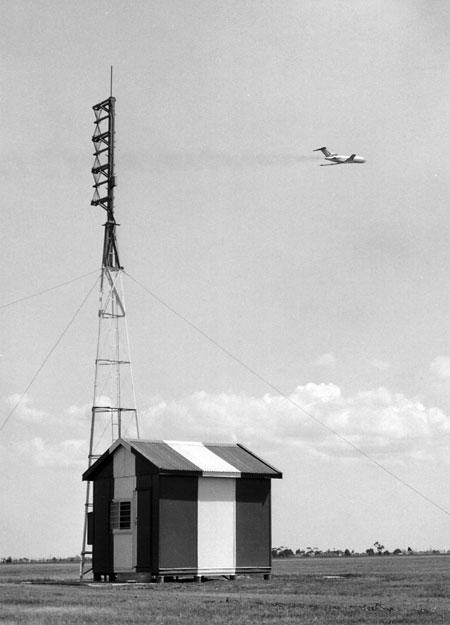
\includegraphics[width=0.4\textwidth]{Imagenes/06.04.dme.imagenes/Aus-DME-installation-external.jpg}
  \label{fig:DME(D).instalacion.tierra}
}
\hspace{3mm}
     \subfigure[Instalaci\'on terrestre de un DME actual
{\tiny fuente: \url{http://
http://www.systemsinterface.com/Systems/Navaids/DME/tabid/440/Default.aspx
}}]
{
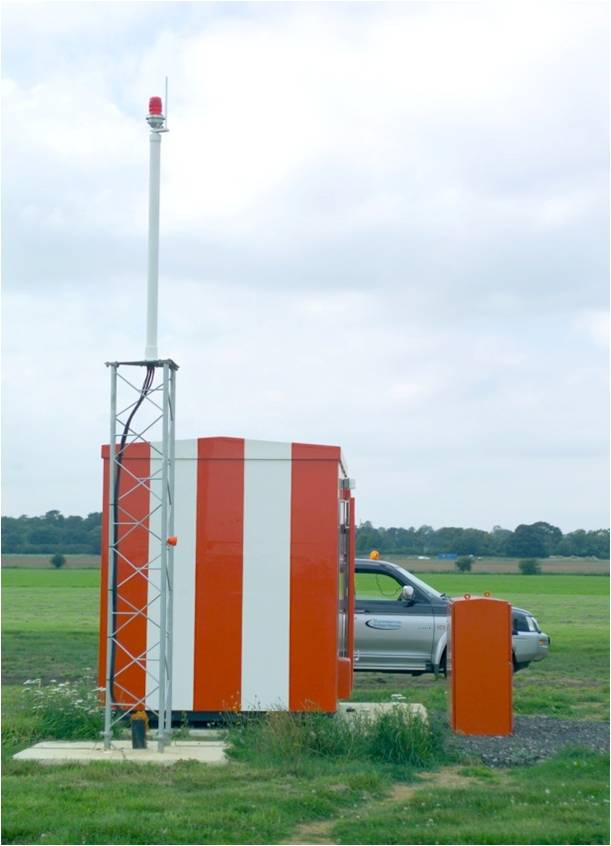
\includegraphics[width=0.4\textwidth]{Imagenes/06.04.dme.imagenes/DME-actual.jpg}
  \label{fig:DME(D).instalacion.tierra}
}
 
 \end{figure}

\begin{figure}[!h]
  \centering
  \includegraphics[width=0.6\textwidth]{Imagenes/06.04.dme.imagenes/DMEtheoryGround.gif}
  \caption{Diagrama de bloques del Equipo DME en tierra {\tiny 
fuente: \url{http://
www.thalesatminc.com/Technology/DME415.htm
}}}
  \label{fig:DME.equipo.tierra.diagrama.bloques}
\end{figure}

\subsection{Equipo de a bordo }
\label{sec:DME.equipo.a.bordo}

\subsubsection{Indicador DME}
\label{sec:DME.indicador}

DME permite a las aeronaves para establecer su rango a la estaci\'on de tierra: La distancia en millas n\'auticas, la velocidad en nudos de tierra, el tiempo de vuelo a la estaci\'on en cuesti\'on de minutos. 

La interpretaci\'on es directa. El piloto puede leer directamente desde el receptor de la distancia, y en su caso la velocidad del recorrido y el tiempo para la estaci\'on.  En la Figura \ref{fig:DME.equipo.a.bordo} puede apreciarse un equipo comercial y en la Figura \ref{fig:DME.instalacion.a.bordo} la informaci\'on brindada por el equipo.


\begin{figure}[!h]
  \centering
  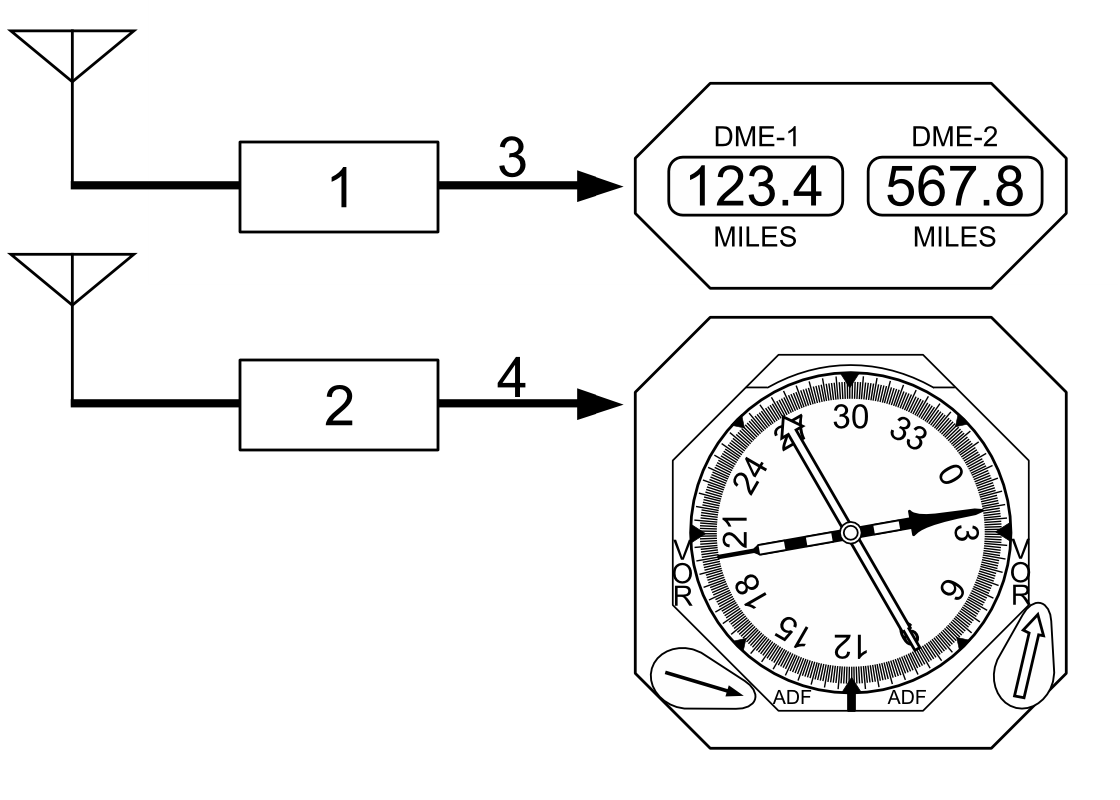
\includegraphics[width=0.6\textwidth]{Imagenes/06.04.dme.imagenes/DME_VOR_avionics.PNG}
  \caption{Equipo de DME junto con uno de ADF 
{\tiny fuente: \url{http://
en.wikipedia.org/wiki/Distance_measuring_equipment
}}
}
  \label{fig:DME.instalacion.a.bordo}
\end{figure}


\subsubsection{Localizaci\'on de la antena en la aeronave}
\label{sec:DME.localizacion.antena.aeronave}

La antena DME de la estaci\'on emite una se\~nal de radiofrecuencia VHF en todas direcciones, que es recibida por el equipo VOR de cualquier aeronave que se encuentre dentro del rango de alcance (max. unos 240 km) y tenga sintonizada la frecuencia de dicha estaci\'on (que puede variar de 108 a 118 MHz modulada en AM). En la Figura \ref{fig:fig:DME.antena.ubicacion.en.el.avion} puede observarse la ubicaci\'on m\'as com\'un de la antena para el equipo DME en la aeronave.

\begin{figure}[!htb]
  \subfigure[Equipo de a bordo
{\tiny fuente: \url{http://
http://http://www.futureplatone.com/es/avionica/267-elite-ap-4000-dme-module.html
}}
]{
  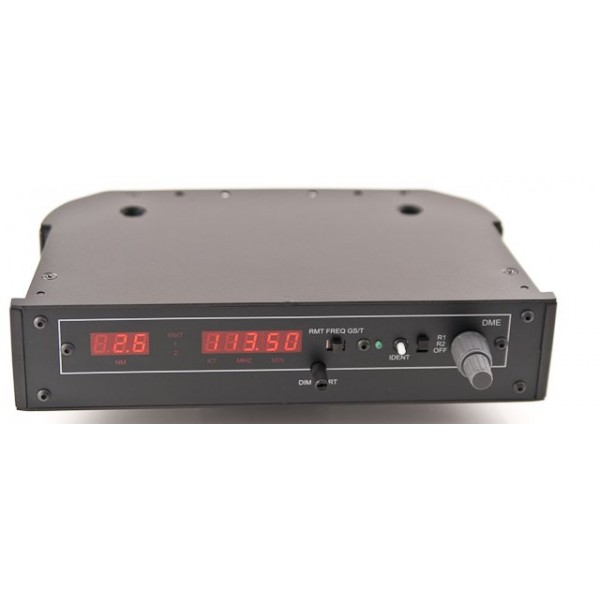
\includegraphics[width=0.4\textwidth]{Imagenes/06.04.dme.imagenes/elite-ap-4000-dme-module.jpg}
\label{fig:DME.equipo.a.bordo}
}
\hspace{3mm}
  \subfigure[
Localizaci\'on de la antena en la aeronave
{\tiny fuente: \url{http://
www.taringa.net/posts/ciencia-educacion/13993518/equipo-medidor-de-distacia-_dme_.html
}}
]{
  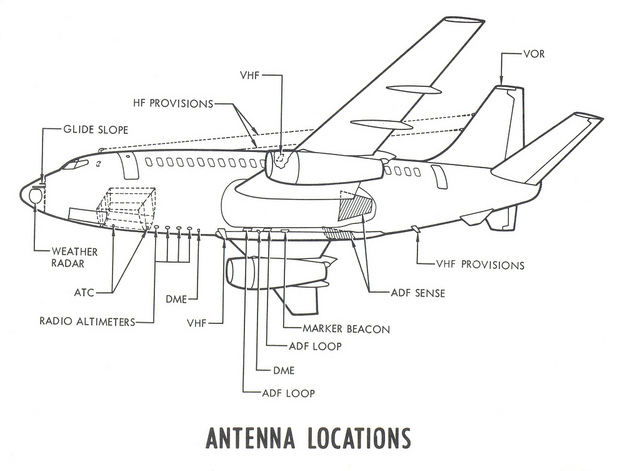
\includegraphics[width=0.6\textwidth]{Imagenes/06.04.dme.imagenes/antenas-en-el-avion.jpg}
\label{fig:fig:DME.antena.ubicacion.en.el.avion}
}
\end{figure}



\subsection{Mediciones err\'oneas}
\label{sec:DME.mediciones.erroneas}

Hay que tener siempre en cuenta que la distancia medida por el DME es la distancia real en l\'inea recta entre el avi\'on y la estaci\'on, que variar\'a dependiendo de la altitud a la que nos encontremos. Para hacernos una idea, aunque nos encontremos sobrevolando en DME, no indicar\'a cero sino que nos dar\'a una lectura en millas n\'auticas de la altitud a la que nos encontramos. Para obtener la distancia real sobre el suelo, que es la que nos interesar\'a a la hora de planificar el vuelo, habr\'a que aplicar el teorema de Pit\'agoras: $\text{Hipotenusa}^2 = \text{Altura}^2+\text{Distancia}^2$.


\begin{figure}[!htb]
  \centering
  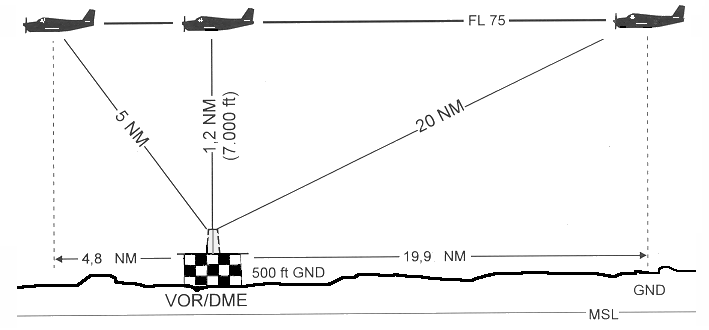
\includegraphics[width=0.7\textwidth]{Imagenes/06.04.dme.imagenes/DME_overfly.png}
  \caption{Mediciones del DME. {\tiny fuente: \url{http://www.langleyflyingschool.com/Pages/CPGS\%20Radio\%20Navigation.html
}}
}
  \label{fig:DME.mediciones}
\end{figure}

En la f\'ormula habr\'a que igualar las distancias a la misma medida (lo m\'as sencillo es convertir la altura a millas n\'auticas), siendo la hipotenusa del tri\'angulo la distancia medida por el DME,  nuestra \emph{Altura} respecto a la de la estaci\'on y \emph{Distancia} la existente sobre el suelo para sobrevolar la estaci\'on.

Si el equipo dispone de la posibilidad del c\'alculo de la ground speed (GS) o del tiempo estimado (ETE) para llegar a la estaci\'on habr\'a que saber que el equipo lo calcula seg\'un la velocidad a la que nos acercamos a la estaci\'on y que por lo tanto s\'olo ser\'a una medida fiable si nos dirigimos a ella directamente. Si hici\'eramos un arco DME (girar alrededor de un DME a una distancia fija) el equipo entender\'ia que no nos estamos acercando y por lo tanto llegar\'ia a indicar 0 nudos de GS si hacemos la maniobra con total precisi\'on independientemente de la velocidad real a la que nos desplazamos. Una forma muy sencilla de ver esto es volar cerca de un DME sin dirigirse a \'el y comparar la velocidad que nos indica con la GS que nos marca el GPS, si disponemos de uno.

\section{Exactitud del sistema}
\label{sec:DME.exactitud}

La exactitud del sistema DME es normalmente de 100 a 300 m. Un valor t\'ipico de $0.1$ NM (185 m) se da a veces como referencia. 

Las fuentes de error son:
\begin{itemize}
\item Inexactitudes debidas al equipo
  \begin{itemize}
  \item los $50\,\mu$ seg de retardo tras la recepci\'on de una interrogaci\'on
    est\'an sujetos a un error de $\pm 1\,\mu$ seg
  \item Detecci\'on por parte del receptor
  \end{itemize}
\item Reflexiones (fen\'omeno de   multicamino o multi-path)
\end{itemize}

Las tolerancias aceptables en las indicaciones del DME en la cabina son de $\pm 0.5$\,NM o 3\% de la distancia, tomandose el valor mayor.

\section{Ventajas y desventajas del sistema}
\label{sec:DME.ventajas.y.desventajas}

\begin{tabular}{|m{0.45\textwidth}|m{0.45\textwidth}|} \hline
	\centering \textbf{Ventajas} & 
	\multicolumn{1}{c|}{\textbf{Desventajas}} \\ \hline
  \begin{itemize}
  \item Proporciona a la aeronave informaci\'on de distancia a la
    estaci\'on terrestre.
  \item F\'acilmente asociable a CVOR, DVOR e ILS.
  \item M\'as de 200 interrogaciones simult\'aneas.
  \item Transpondedor \'integramente programable.
  \item Compatible con antenas sectoriales y omnidireccionales.
  \item Totalmente supervisable y controlable a distancia.
  \end{itemize}
	&
        \begin{itemize}
        \item El sistema puede saturarse cuando hay muchas aeronaves dentro del alcance del radiofaro. 
        \item 	Algunos DME asociados con el ILS pueden requerir disposiciones especiales para su protecci\'on contra la interferencia. 
        \end{itemize}
        \\ \hline
\end{tabular}





%
%  Asi se citan las direcciones web
%
%Example usage
%
%In the preamble:
%---------------
%
%\usepackage{url}
%
%% Define a new 'leo' style for the package that will use a smaller font.
%\makeatletter
%\def\url@leostyle{
%  \@ifundefined{selectfont}{\def\UrlFont{\sf}}{\def\UrlFont{\small\ttfamily}}}
%\makeatother
%
% Now actually use the newly defined style.
%
%\urlstyle{leo}
%
%
%In a BibTeX entry:
%------------------
%
%@misc{
%    c.elmohamed,
%    author = "Saleh Elmohamed",
%    title = "Examples in {H}igh {P}erformance {F}ortran",
%    howpublished = "Website",
%    year = {1996},
%    note = {\url{http://www.npac.syr.edu/projects/
%                    cpsedu/summer98summary/ examples/hpf/hpf.html}}
%}




